\chapter{ROOTを始めよう}
\label{chapter_Install}
\section{ROOTのインストールと初期設定}
\label{sec_ROOT_install}
\subsection{必要な環境}
本書を読み進めるためには、当然ながらROOTを実行するためのコンピュータ環境が必要です。ROOTがサポートするOSは多岐にわたりますが、2016年現在、Mac OS XかLinuxを使用するのが、この業界では標準です。そのため本書ではOS XかLinuxの使用を前提とします\footnote{WindowsやSolarisでもROOTは動作します。}。どちらかのOSを使う限り、作業内容はほぼ同じはずです。本書に書かれているROOTでの作業を全て行うためには、自分のコンピュータにコンパイラ(compiler)がインストールされている必要があります\footnote{GCCやClangといったコンパイラについての説明や、そのインストール方法は本書の範囲内ではありません。GCCやClangのインストール方法が分からなければ、「GCC インストール Linux」「Clang インストール Mac」などで検索して下さい。}。

ある程度のコマンドラインの使用経験を前提としていますので、\texttt{ls}や\texttt{cd}のような単純なコマンド、「スーパーユーザー」、「管理者」、「ディレクトリ」といった用語の説明は省略します。この章の記述は、コマンドライン操作の初心者には不親切かもしれません。しかし、この章を読み進めることができなければ、恐らくROOTを使いこなせるようにもなりません。コンパイルができなかった、ROOTがうまく起動しなかった、この章に書いてあることが分からなかったという場合は、自力でインターネットや書籍、研究室の同僚を頼りに解決して下さい。

\subsection{ダウンロード}
\label{subsec_download}
ROOTは\url{http://root.cern.ch/}からダウンロードすることができます。既にコンパイルされているバイナリ版と、コンパイルされていないソースコードがあります。前者はコンパイルする必要がないので簡単ですが、本書では教育目的のため、ソースコードをダウンロードして、自分でコンパイルすることにします。

2016年4月時点で、ROOT 6 の最新バージョン6.06/02です。バージョン5からバージョン6に変わるとき、大きな変更がありました。そのため、研究室によってはバージョン5系列を使っている人もまだまだ多いと思います。ROOT 5 では、バージョン 5.34/36 が最新です。最初の数字はメジャーバージョン、次の数字は大きな機能追加ごとに増えるマイナーバージョン、スラッシュの後ろの数字はバグフィックスを示す番号です。

どのバージョンを選択するかは研究室の計算機環境や実験グループの解析ソフトなどに依存しますが、本書では6.06/02を前提として話を進めます。

上記URLを辿ると、ダウンロードのページがあります。リンクをクリックしてダウンロードすることも可能ですが、ここでは直接ターミナルからダウンロードします。
\begin{lstlisting}[language=bash]
$ cd ~
$ curl -O https://root.cern.ch/download/root_v6.06.02.source.tar.gz
\end{lstlisting}
などとして、好きなディレクトリにダウンロードして下さい。今の例では、\texttt{root\_v6.06.02.source.tar.gz}がホームディレクトリ(\texttt{\~})に保存されます\footnote{ホームディレクトリとは、ユーザごとのファイルを置くためのディレクトリのことです。例えば Linux だと、ユーザ\texttt{oxon}の場合は\texttt{/home/oxon}が一般的にホームディレクトリになります。OS X の場合は\texttt{/Users/oxon}になります。これらは省略して\texttt{{\textasciitilde}oxon}、\texttt{\textasciitilde}、\texttt{\$HOME}と書かれることがあります。}。

\subsection{\texttt{configure}を使ったコンパイル}
\label{subsec_compile_configure}
ROOTのコンパイル作業やインストール先は、好きな場所でやって構いません。もしあなたがコンピュータの管理者権限を持っているならば、\texttt{/usr/local}の下にインストールするのが標準的です。次のように、ターミナルから好きなディレクトリに移動し、ソースコードを展開して下さい\footnote{この例のように、先頭に\texttt{\$}がついている行は、ターミナルで入力していることを表します。実際にターミナルから入力する内容は、\texttt{\$}とその直後の半角スペースを取り除いた内容ですので、注意して下さい。}\footnote{管理者権限を持っていなかったり、\texttt{sudo}コマンドを使用できない場合、一般ユーザでもインストール可能なディレクトリを選択してください。}。
\begin{lstlisting}[language=bash]
$ cd /usr/local
$ sudo tar zxvf ~/root_v6.06.02.source.tar.gz
\end{lstlisting}

\texttt{root-6.06.02}という名前のディレクトリが作成されるので、そこに移動してコンパイルを行います。一般的なソフトウェアのコンパイルと同様に、\texttt{configure}スクリプトを実行します。

\begin{lstlisting}[language=bash]
$ cd root-6.06.02
$ ./configure
\end{lstlisting}

ここで色々とターミナルに出力されますが、最後に次のような表示が出れば\texttt{configure}は成功です。もし何かしらのエラーが表示される場合、ROOTのビルドに必要な他のコマンドやライブラリがインストールされていないことが考えられます。表示されたエラーをよく読み、原因が何かを考えて対応しましょう。
\begin{lstlisting}[language=bash]
Enabled support for asimage, astiff, bonjour, builtin_afterimage, builtin_ftgl, builtin_freetype, builtin_glew, builtin_llvm, libcxx, cocoa, explicitlink, fink, fftw3, fitsio, gviz, genvector, krb5, ldap, mathmore, memstat, opengl, python, rpath, search_usrlocal, shared, sqlite, ssl, tmva, vdt, xml.

To build ROOT type:

   make 
\end{lstlisting}
では、出力の指示に従って\texttt{make}と打ってみましょう。
\begin{lstlisting}[language=bash]
$ make
\end{lstlisting}
\texttt{make}を実行した後に\texttt{make install}を実行したくなりますが、本書の説明通りに作業を進める場合は、別にやる必要はありません。複数コアのCPUを使える場合には、コアの数に応じて最後の行に\texttt{-j 4}のような引数をつけると、コンパイルが早くなります。うまくコンパイルが全て完了すると、以下のような表示が最後に出るはずです。
\begin{lstlisting}
root [0] 
Processing hsimple.C...
hsimple   : Real Time =   0.07 seconds Cpu Time =   0.05 seconds
(TFile *) 0x7fb0fae560c0
 
   ============================================================
   ===                ROOT BUILD SUCCESSFUL.                ===
   === Run 'source bin/thisroot.[c]sh' before starting ROOT ===
   ============================================================
\end{lstlisting}

ここまででエラーが出なければ成功です。もし不運にもエラーが出てしまった人は、コンパイル済みのバイナリをダウンロードしましょう。以下は、OS X版をダウンロードした場合の例です。コンパイル済みのものは最新版に更新されていない可能性もあるため、やはり自分でコンパイルするのが確実です。
\begin{lstlisting}[language=bash]
$ cd ~
$ curl -O https://root.cern.ch/download/root_v6.06.02.macosx64-10.11-clang70.tar.gz
$ cd /usr/local
$ sudo tar zxvf ~/root_v6.06.02.macosx64-10.11-clang70.tar.gz
\end{lstlisting}
コンパイル済みのバイナリは、全ての環境用に配布されているわけではありません。ROOTのダウンロードページ\footnote{\url{https://root.cern.ch/content/release-60602}}から、自分の環境に対応したものをダウンロードしましょう\footnote{2016年4月現在、OS X 10.9(Mavericks)、10.10(Yosemite)、10.11(El Capitan)、RHEL6クローン(Scientific Linux 6など)、RHEL7クローン(CentOS 7など)などにバイナリ配布があります。}。

\subsection{\texttt{CMake}を使ったコンパイル}
\label{subsec_compile_cmake}
最近の\texttt{ROOT}では、\texttt{configure}コマンドではなく\texttt{cmake}コマンド\footnote{\url{https://cmake.org/}}を使ってビルドすることができます。これは\texttt{Geant4}でも同様で、最近のソフトウェアの流れです。\texttt{CMake}はまだ完全に市民権を得たわけではありませんが、徐々に浸透しつつあるため、興味のある人は\texttt{CMake}でビルドしてみるのも良いでしょう。

\texttt{yum}、\texttt{MacPorts}、\texttt{homebrew}などで、まずは\texttt{CMake}を導入します。その後の流れは以下の通りです\footnote{\texttt{cmake\_build}というディレクトリ名は好きなもので構いません。}。

\begin{lstlisting}[language=bash]
$ cd /usr/local
$ sudo tar zxvf ~/root_v6.06.02.source.tar.gz
$ mkdir root-6.06.02/cmake_build
$ cd root-6.06.02/cmake_build
$ cmake ..
\end{lstlisting}

問題がなければ、色々とターミナルに出力された最後に以下の表示が出るはずです。
\begin{lstlisting}[language=bash]
-- Configuring done
-- Generating done
-- Build files have been written to: /usr/local/root-6.06.02/cmake_build
\end{lstlisting}

あとは、\texttt{configure}のときと同様に\texttt{make}を実行します。
\begin{lstlisting}[language=bash]
$ make
\end{lstlisting}

\subsection{最低限の初期設定}
\label{subsec_settings}
ソースをコンパイルしたり、バイナリ版をダウンロードしただけではROOTは使えるようになりません。ROOTの実行ファイルやライブラリの場所を設定する必要があります。以下の3行を\texttt{\~{}/.bashrc}に書き足して下さい\footnote{もし\texttt{/usr/local/root}以外の場所にインストールした場合は、ディレクトリを適宜変更してください。}。
\begin{NoFloat}
\lstinputlisting[language=bash]{src/bashrc.sh}
\end{NoFloat}
もし\texttt{CMake}を使った場合は次のようになります。
\begin{NoFloat}
\lstinputlisting[language=bash]{src/bashrc_cmake.sh}
\end{NoFloat}

これらは、ログインシェルに\texttt{bash}を使っている人の場合です。もしzshを使っている場合は、\texttt{\~{}/.zshrc}に書いて下さい。書き終わったら、
\begin{lstlisting}[language=bash]
$ source ~/.bashrc
\end{lstlisting}
とするか、新しいターミナルを開いてください。もし\texttt{csh}や\texttt{tcsh}を使っている場合は、\texttt{\~{}/.cshrc}や\texttt{\~{}/.tcshrc}に以下の3行を書き足して下さい。
\begin{NoFloat}
\lstinputlisting[language=csh]{src/cshrc.sh}
\end{NoFloat}
そして同様に
\begin{lstlisting}[language=bash]
$ source ~/.cshrc
\end{lstlisting}
とするか、新しいターミナルを開きましょう。\texttt{source}コマンドを実行する必要があるのは、初めて\texttt{.bashrc}や\texttt{.cshrc}の設定をROOT用に変更したときだけです。次にターミナルを開くときには自動的に処理されますので、\texttt{source}コマンドを打つ必要はありません。

以上の設定で、使用しているシェルの環境変数の内容が更新されます。\texttt{ROOTSYS}という変数が追加され(これは\texttt{/usr/local/root}を指しているはずです)、\texttt{PATH}、\texttt{LD\_LIBRARY\_PATH}、\texttt{PYTHONPATH}などが\texttt{ROOTSYS}以下のディレクトリを含むように変更されています。

\subsection{動作確認}

それでは早速、ROOTを起動してみましょう。
\begin{lstlisting}[language=bash]
$ root
\end{lstlisting}
と打ってみて下さい。図\ref{fig_splash}が画面に現れるとともに、ターミナルには以下のように出力されます。
\begin{lstlisting}
   ----------------------------------------------------------------
  | Welcome to ROOT 6.06/02                    http://root.cern.ch |
  |                                   (c) 1995-2014, The ROOT Team |
  | Built for macosx64                                             |
  | From heads/master@v6-07-02-437-gb06340c, Mar 02 2016, 19:01:57 |
  | Try '.help', '.demo', '.license', '.credits', '.quit'/'.q'     |
   ----------------------------------------------------------------

root [0] 
\end{lstlisting}
もしも\texttt{root}というコマンドが見つからないというエラーが出た場合は、\texttt{PATH}環境変数の設定が正しく行われていません。またライブラリが見つからないというエラーが出た場合は、\texttt{LD\_LIBRARY\_PATH}の設定が正しく行われていません。\texttt{.bashrc}や\texttt{.cshrc}に打ち間違いがないか再確認しましょう。

最後の行の
\begin{lstlisting}
root [0]
\end{lstlisting}
は、ROOTが入力待ちをしている状態です。これをプロンプト(prompt)と呼びます。ここに色々なコマンドを打つことによってROOTを操作します。ひとまず
\begin{lstlisting}
root [0] .q
\end{lstlisting}
と入力しましょう(Quitのqです)。これでROOTが終了します。ここまでで、ROOTの起動と終了ができるようになりました。毎回起動の度に起動画面とバージョン情報が出るのが鬱陶しい場合、引数をつけて
\begin{lstlisting}[language=bash]
$ root -l
\end{lstlisting}
として起動しましょう。すぐにROOTのプロンプトが表示されるはずです。毎回引数をつけるのが面倒な場合は、
\begin{lstlisting}[language=bash]
alias root="root -l"
\end{lstlisting}
を\texttt{\~{}/.bashrc}に、もしくは
\begin{lstlisting}[language=csh]
alias root "root -l"
\end{lstlisting}
を\texttt{\~{}/.cshrc}に書き足すとよいでしょう。

\begin{figure}
  \centering
  
\includegraphics[width=12cm]{fig/splash6.png}
  \caption{ROOTの起動画面}
  \label{fig_splash}
\end{figure}

\subsection{チュートリアルで遊ぶ}
\label{subsec_tutorial}
ROOTで作業できる内容は様々です。何ができるかを言葉で説明するよりは、どんな図を作ることが可能か眺めるのが手っ取り早いでしょう。まずは、ROOTのチュートリアルで遊んでみましょう。\texttt{\$ROOTSYS/tutorials}には様々な例題が置かれています。このディレクトリに移動すると、少し起動後の出力が変わります。
\begin{lstlisting}[language=bash]
$ cd $ROOTSYS/tutorials
$ root

Welcome to the ROOT tutorials


Type ".x demos.C" to get a toolbar from which to execute the demos

Type ".x demoshelp.C" to see the help window

==> Many tutorials use the file hsimple.root produced by hsimple.C
==> It is recommended to execute hsimple.C before any other script

root [0] .x demos.C
\end{lstlisting}
最後の行は、\texttt{demos.C}という名前のファイルを実行せよという命令です(eXecuteのx)。\texttt{.q}に続いて、基本中の基本コマンドなので覚えましょう。このような複数のROOTの命令が記述されたファイルを、スクリプト(script)やマクロ(macro)と呼ぶことがあります\footnote{ROOTはCINTというライブラリによって、C++のソースファイルをコンパイルすることなく実行することが可能です。そのため、shell、Python、Perlなどのスクリプト言語と同様にスクリプトと呼びます。「ROOTソース」と言う場合にはROOT本体のソースコードを、「ROOTスクリプト」と言う場合には解析用にユーザが書いたプログラムを指すことが多いと思います。}。

このコマンドを実行すると、いくつかボタンが表示されるはずです。このうち、「hsimple」と書かれたボタンをクリックしてみましょう。図\ref{fig_hsimple}のようなウインドウが表示されるはずです。他にも沢山の例が実行可能ですので、全てのボタンをクリックして遊んでみて下さい。終了のときは、やはり\texttt{.q}と打ちます。

\begin{figure}
  \centering
  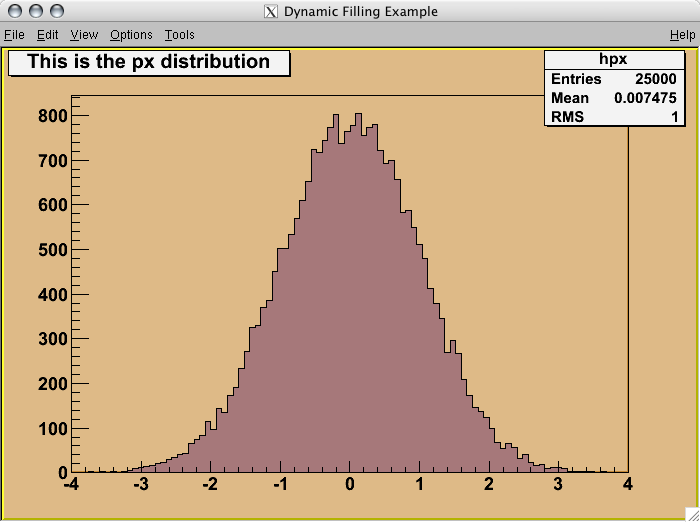
\includegraphics[width=12cm]{fig/hsimple.png}
  \caption{hsimpleの実行結果}
  \label{fig_hsimple}
\end{figure}

もし、あなたのアカウントが\texttt{\$ROOTSYS/tutorials}に書き込み権限を持たない場合、\texttt{hsimple.root}を開けないというエラーが出るでしょう。そのような場合は、書き込み権限を持つユーザで作業をするか、\texttt{\$ROOTSYS/tutorials}をディレクトリごと自分のホームディレクトリの下にコピーして、そこで作業をしましょう。

\section{ROOTの操作に慣れる}

まずは、簡単な例を走らせることでROOTの操作方法に慣れましょう。ここでは、標準偏差(standard deviation)$\sigma=1$の正規分布(normal distribution、Gaussian distribution)に従った、標本の大きさ(sample size)$n=10000$のヒストグラム(histogram)を作ってみます。

\subsection{コマンドラインからの操作}
まずはROOTを起動し、
\begin{lstlisting}[language=c++]
root [0] TH1D* hist = new TH1D("myhist", "Gaussian Histogram (#sigma = 1)", 50, -5, 5)
root [1] hist->FillRandom("gaus", 10000)
root [2] hist->Draw()
Info in <TCanvas::MakeDefCanvas>:  created default TCanvas with name c1
\end{lstlisting}
という3行を打ってみて下さい。最後の行はROOTが自動的に出力しますが、エラーではないので今は気にしないで下さい。図\ref{fig_first_script}のような実行結果が画面に現れます。
\begin{figure}
  \centering
  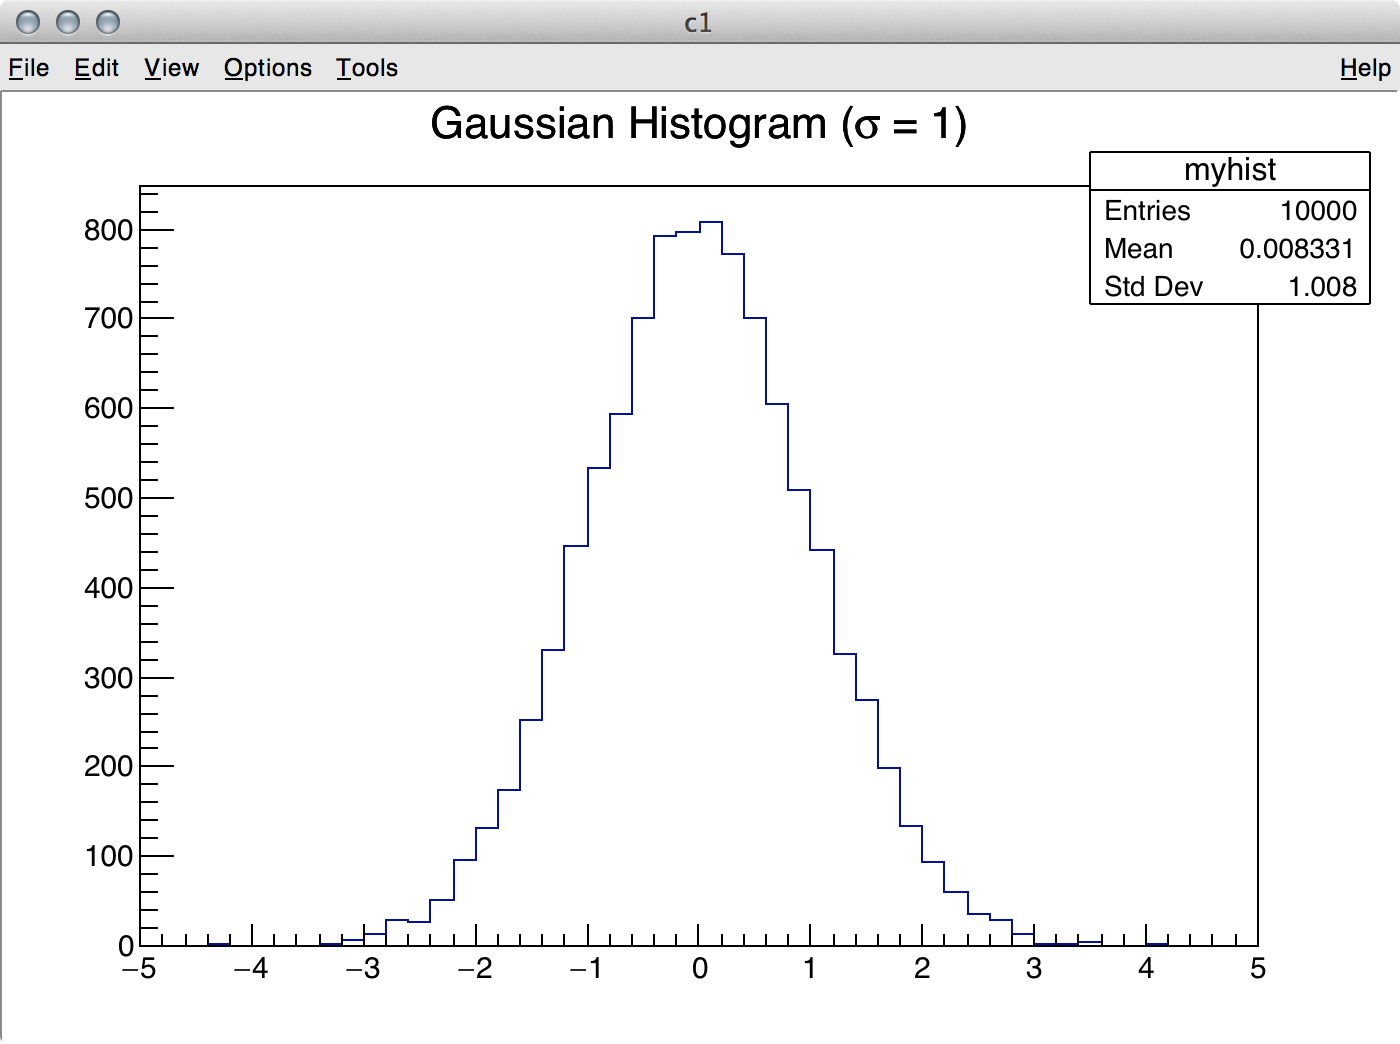
\includegraphics[width=12cm]{fig/first_script.png}
  \caption{標準偏差$\sigma=1$、標本の大きさ$n=10000$のヒストグラム}
  \label{fig_first_script}
\end{figure}

このままでは何が起きたか分からないので、簡単に説明します。C++やプログラミングの用語が混ざりますが、各自で調べつつ読んで下さい。これらの3行は、実はC++の言葉で書かれています。まず
\begin{lstlisting}[language=c++]
root [0] TH1D* hist = new TH1D("myhist", "Gaussian Histogram (#sigma = 1)", 50, -5, 5)
\end{lstlisting}
の部分では、\texttt{TH1D}クラス(class)のインスタンス(instance)を作成しています。このインスタンスの名前は、この例ではhistとしています。\texttt{*}や\texttt{new}は、おまじないだと思っておいて下さい\footnote{コンピュータ関連の説明文書の中で、「おまじない」という言葉がたまに出てきます。「それが何者であるか(今は)理解する必要はないが、こうしておくと正しく動作する」ようなものを「おまじない」と呼ぶ習慣があります。とりあえず気にするなということです。}。このhistが、ヒストグラムの実体になります。\texttt{"myhist"}や\texttt{"Gaussian Histogram (\#sigma = 1)"}という文字列、$50$、$-5$、$5$という数字が図\ref{fig_first_script}のどの箇所に対応するか、自分で考えて下さい。このヒストグラムは、この時点では作りたてなので、当然中身は空っぽです。そこで
\begin{lstlisting}[language=c++]
root [1] hist->FillRandom("gaus", 10000)
\end{lstlisting}
として、正規分布に従う数字$10000$個を乱数で発生させ、ヒストグラムに詰めています。最後に
\begin{lstlisting}[language=c++]
root [2] hist->Draw()
\end{lstlisting}
としてヒストグラムを画面に描画させています。

\subsection{スクリプトを使った操作}
今回の例はたったの3行ですので入力は簡単です。しかし、このようなヒストグラムを何百回と繰り返し作成することを想像してみて下さい。実際のデータ解析では、取得した大量のデータに同じ処理をしたい場合があります。そのようなときに、同じコマンドを何度も繰り返し入力するのは非効率的です。そこで、先ほどの3行を1つのファイルにまとめて書いてしまいましょう。コード\ref{code_first_script}の内容を入力したテキストファイルを\texttt{first\_script.C}というファイル名で好きな場所に保存して下さい\footnote{日本語の文章の書き方は個人で色々な癖があるように、プログラミング言語の記述にも人それぞれの流儀があります。本書で採用しているコードの流儀は、かなり著者の好みが反映されています。}。このようなファイルを、ROOTのスクリプトファイル、マクロファイルなどと呼びます。
%\begin{NoFloat}
\lstinputlisting[language=c++,float=tb,caption=\texttt{first\_script.C},label=code_first_script,numbers=left]{src/first_script.C}
%\end{NoFloat}

\texttt{first\_script.C}を保存したディレクトリに移動し、その場所でROOTを立ち上げ、次の行を実行します。
\begin{lstlisting}[language=c++]
root [0] .x first_script.C
Info in <TCanvas::MakeDefCanvas>:  created default TCanvas with name c1
\end{lstlisting}
先ほどと同様の実行結果(図\ref{fig_first_script})が得られるはずです。ここで、再び\texttt{.x}というコマンドが登場しました。\texttt{first\_script.C}を実行せよという意味です。\texttt{first\_script.C}に書かれた内容が逐一実行されたため、図\ref{fig_first_script}の結果が得られたわけです。

1度実行するだけでは、せっかく別ファイルにしたありがたみが分かりません。そこでコード\ref{code_first_script2}のように少し書き直して、\texttt{first\_script2.C}というファイルを作成してみて下さい。
%\begin{NoFloat}
\lstinputlisting[language=c++,float=tb,caption=\texttt{first\_script2.C},label=code_first_script2,numbers=left]{src/first_script2.C}
%\end{NoFloat}
先ほどと同様に実行してみましょう。ただし今回は
\begin{lstlisting}[language=c++]
root [0] .x first_script2.C(500, 100000)
Info in <TCanvas::MakeDefCanvas>:  created default TCanvas with name c1
\end{lstlisting}
としてみます。少し先ほどの例とは表示されるヒストグラムが変化したはずです。2つの数字を何通りか試して、何が起きてるか確かめて下さい。何度も実行すると、
\begin{lstlisting}[language=c++]
Warning in <TROOT::Append>: Replacing existing TH1: myhist (Potential memory leak).
\end{lstlisting}
というROOTの警告(warning)が出るはずですが、今は無視しましょう。

ここまでの作業を振り返ってみます。最初にROOTのプロンプトから入力した行は3行だけでしたが、コード\ref{code_first_script}と\ref{code_first_script2}では上に2行、下に1行追加され、合計6行になっています。この余計な部分を含めて、関数(function)と呼びます。\texttt{void}はおまじないです。\texttt{int nbins}や\texttt{int nevents}の部分は、引数(argument)と呼ばれるものです。このように特定の機能を関数化することによって、汎用性が高くなります。

ROOTのスクリプトファイルでは、そのファイル名と同一の関数がファイル内に存在すると、その関数が実行されます。したがって、コード\ref{code_first_script2}に書いた関数名を\texttt{first\_script2}から例えば\texttt{foo}\footnote{\texttt{foo}や\texttt{bar}というのは、とりあえずの適当な名前として、プログラミングの話題をするときによく出てきます。日本語だと、「ほげ」や\texttt{hoge}という単語もよく使われます。}に変更してしまうと、
\begin{lstlisting}[language=c++]
root [0] .x first_script2.C(500, 100000)
warning: cannot find function 'first_script2()'; falling back to .L
\end{lstlisting}
というエラーが出てヒストグラムが表示されません。もしファイル名と関数名を別々のものにしたければ、次のやり方も可能です。
\begin{lstlisting}[language=c++]
root [0] .L first_script2.C
root [1] foo(500, 100000)
Info in <TCanvas::MakeDefCanvas>:  created default TCanvas with name c1
\end{lstlisting}
\texttt{.L}コマンドで\texttt{first\_script2.C}をロード(LoadのL)します。そのスクリプトファイルの内容をROOTが呼び出せるようにする作業のことです。\texttt{first\_script2.C}は既にロードされましたので、その中に書かれていた関数\texttt{foo}に引数を与えて直接呼び出すことができます。また、ひとつのスクリプトの中に複数の関数を記述しても問題ありません。ロードした後に、好きな関数を呼び出して下さい。
\subsection{図を保存する}

図\ref{fig_hsimple}や\ref{fig_first_script}の例は、筆者の使用しているOS~X上でスクリーンショットを撮ったものです。論文用の図を作成する場合は、ウインドウ上のリサイズボックスやタイトルバーは必要ありません。\LaTeX\ 文書で一般的に使われる、PDF形式で出力結果を保存してみましょう\footnote{最近の\LaTeX\ 環境では\texttt{latex}コマンドよりも\texttt{pdflatex}コマンドを使用してPDFファイルを生成するのが一般的になりつつあります。そのため、論文出版社もESP形式ではなくPDF形式で図を受け付けています。またEPSよりもPDFのほうがパソコン上での閲覧も楽なため、特に理由がない場合はPDFで保存しましょう。ただし、本書のような日本語文書では\texttt{platex}コマンドがまだまだ使われています。}\footnote{ROOTの生成する横長のPDFには\texttt{/Rotate 90}というタグが含まれており正常に\texttt{dvipdfmx}コマンドや Apple Keynote などで処理できないため、作成した PDF が90度回転して表示されるという問題があります。これを回避するためには、\texttt{can->SaveAs("can.pdf")}などと実行するのではなく、\texttt{can->Print("can.pdf", "pdf Portrait")}と実行しましょう。}。\texttt{first\_script.C}の実行結果が表示されたら、ウインドウ左上にある「File」メニューから「Save As\ldots」を選択し、好きな場所に好きな名前で出力結果を保存しましょう。図\ref{fig_first_script_pdf}は、この手順で図\ref{fig_first_script}をPDF形式で保存し直したものです。このPDF文書を拡大しても、図が綺麗なことが分かります。いくつか保存形式が選べますので、試してみましょう。JPEG形式は図の細部が潰れますので、絶対に使わないでください。GIF形式は最大で256色までしか使用できないので、そのうち凝った図を作る場合にはPNGのほうが良いでしょう。

\begin{figure}
  \centering
  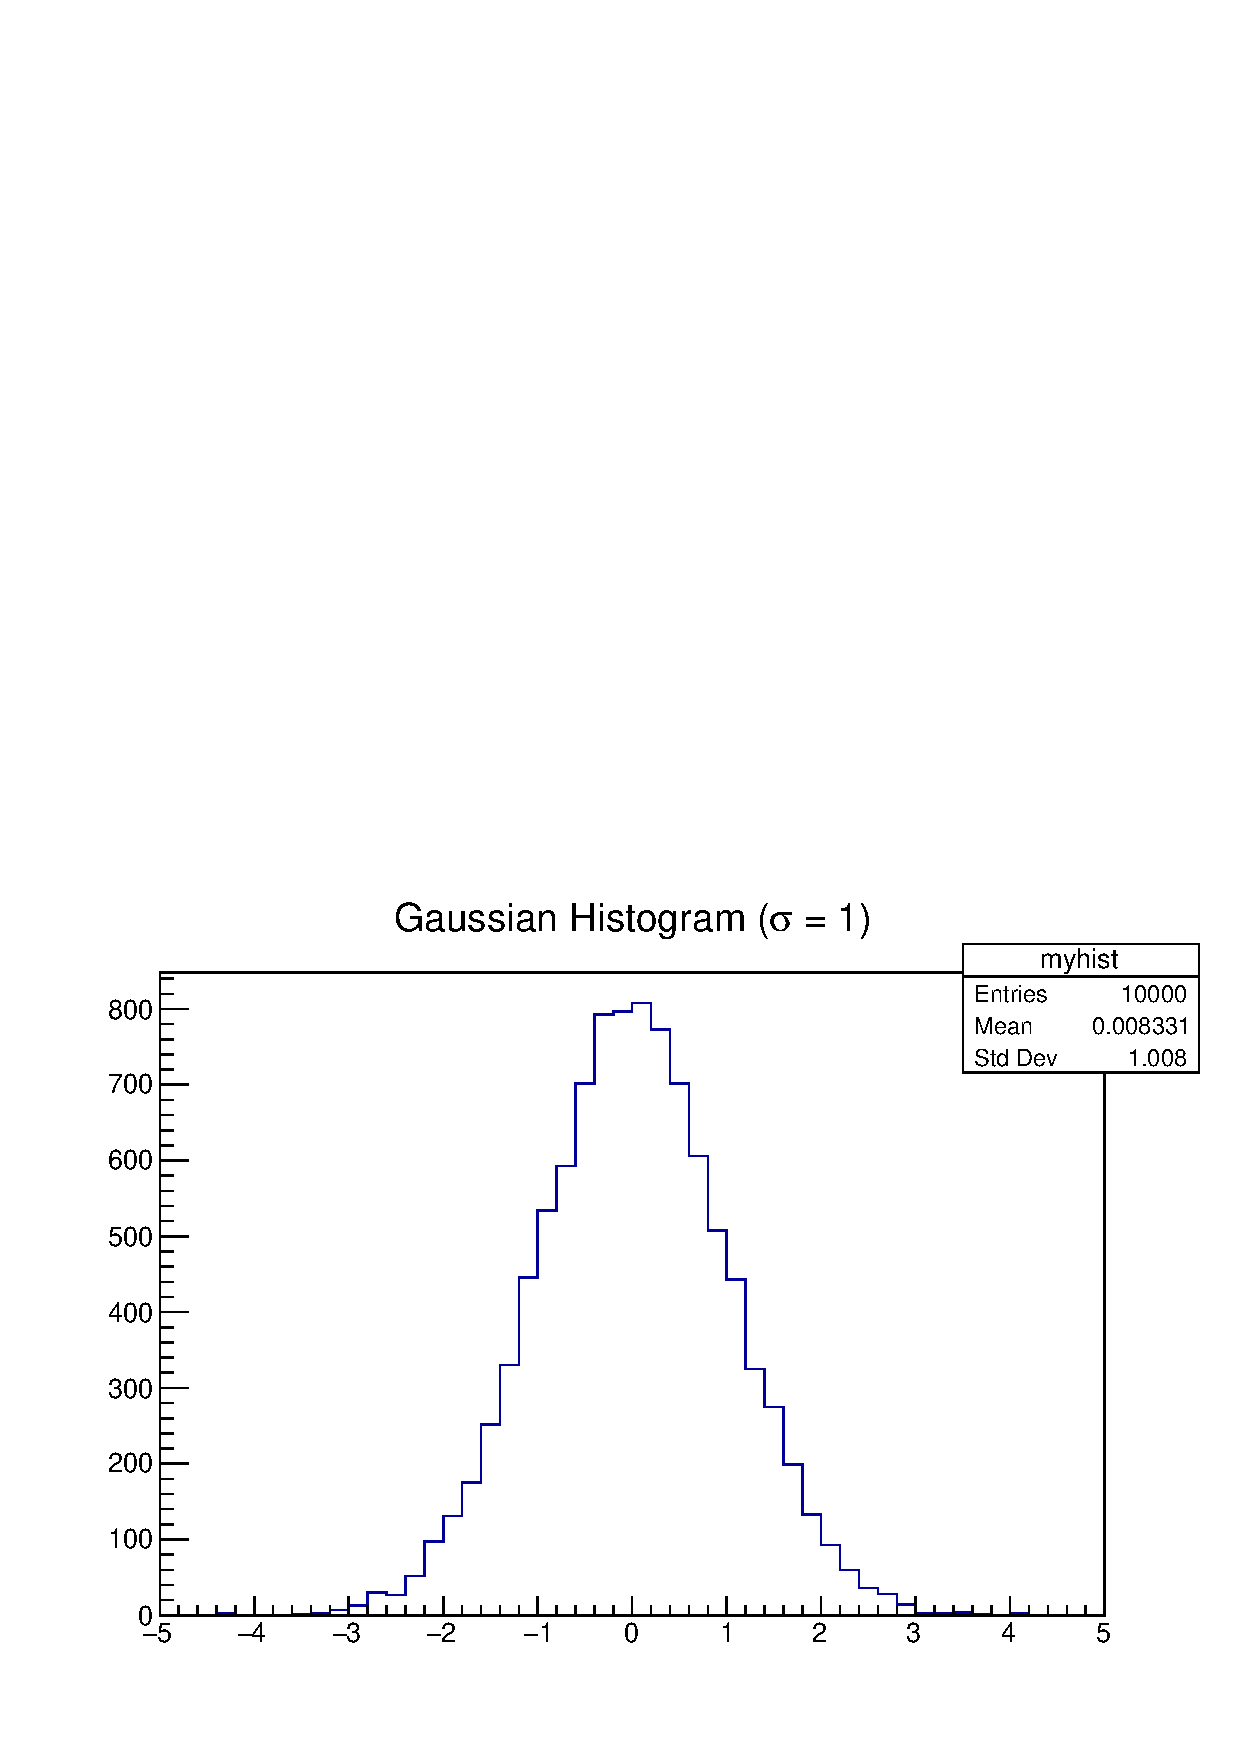
\includegraphics[width=12cm,clip]{fig/first_script_pdf.pdf}
  \caption{図\ref{fig_first_script}を、PDF形式で保存し直したもの}
  \label{fig_first_script_pdf}
\end{figure}

\subsection{タブ補完を使う}

ROOTのプロンプトでコマンドを打つ場合、キーボードのタブキーを押すことで、補完することができます。携帯電話の文字入力の予測変換機能のようなものです。例えば、
\begin{lstlisting}[language=c++]
root [0] TH1D* hist = new TH1D("myhist", "Gaussian Histogram (#sigma=1)", 50, -5, 5)
root [1] hist->FillRandom("gaus", 10000)
root [2] hist->Draw()
Info in <TCanvas::MakeDefCanvas>:  created default TCanvas with name c1
root [3] hi
\end{lstlisting}
とまで入力したところで、タブキーを押してみましょう。自動的に
\begin{lstlisting}[language=c++]
root [3] hist
\end{lstlisting}
と補完されます。次に、
\begin{lstlisting}[language=c++]
root [3] hist->Get
\end{lstlisting}
まで入力して再度タブを押してみましょう。次のような候補が大量に現れるはずです。
\begin{lstlisting}[language=c++]
GetArray
GetAsymmetry
GetAt
GetAxisColor
\end{lstlisting}
これは、インスタンス\texttt{hist}に操作可能な機能のうち、\texttt{Get}で始まるものの一覧です。C++の言葉で言い換えると、クラス\texttt{TH1D}のメンバ関数(member function)のうちゲッター(getter)の一覧です。候補を眺めてみると、\texttt{GetMean}や\texttt{GetStdDev}\footnote{\texttt{GetRMS}というメンバ関数も見つかると思います。ROOTやPAWで「RMS」と言った場合、これは二乗平均ではなく標準偏差を指します。統計学の用語としては不適切なのですが、歴史的理由でRMSという言葉を使い続けているそうです。そのためこの業界ではRMSという用語を間違って覚えている人が沢山いますが、優しく注意してあげて下さい。最近のROOTでは、\texttt{GetRMS}と全く同じ働きをする関数として\texttt{GetStdDev}が用意されています。}というメンバ関数が見つかるはずです。何をする関数か、一目瞭然でしょう。それでは
\begin{lstlisting}[language=c++]
root [3] hist->GetMe
\end{lstlisting}
まで打ち、タブキーを押しましょう。
\begin{lstlisting}[language=c++]
root [3] hist->GetMean
GetMean
GetMeanError
\end{lstlisting}
の2候補にまで絞られます。今は\texttt{GetMean}を試したいので、
\begin{lstlisting}[language=c++]
root [3] hist->GetMean(
\end{lstlisting}
とまで打って再度タブを打ちましょう。今度は、
\begin{lstlisting}[language=c++]
Double_t GetMean(Int_t axis = 1) const
\end{lstlisting}
と表示されます。これは、\texttt{TH1D::GetMean}\footnote{この書き方は、クラス\texttt{TH1D}のメンバ関数\texttt{GetMean}という意味です。}の引数の説明が表示されたものです。引数には整数(integer)値を取り、そのデフォルト(default)値が1だという意味です(1はX軸を意味しています)。何も打たなくてもX軸を指定するデフォルト値が入っているので、
\begin{lstlisting}[language=c++]
root [3] hist->GetMean()
(Double_t) 0.00833117
\end{lstlisting}
と入力します。出力された値は、このヒストグラムの平均値です。ウインドウの右上に既に表示されている値と同一なはずです。同様にして、\texttt{TH1D::GetStdDev()}も試してみましょう。

今度は
\begin{lstlisting}[language=c++]
root [4] hist->Set
\end{lstlisting}
でタブ補完をすると、\texttt{Set}で始まる関数がたくさん表示されます。これらのメンバ関数はセッター(setter)と呼ばれ、ゲッターと対をなすものです。ゲッターとセッター以外にも多くのメンバ関数が存在しますが、ここでは説明しません。試しに
\begin{lstlisting}[language=c++]
root [4] hist->SetLineColor(2)
root [5] hist->SetXTitle("x")
root [6] hist->SetYTitle("Number of Events")
root [7] hist->Draw("e")
\end{lstlisting}
としてみましょう。出力結果と見比べて、何が起きたか分かるはずです。先ほどまでは\texttt{TH1D::Draw}の引数に何も与えていませんでしたが、今度は\texttt{"e"}という引数がついています。なぜこれで動作したかというと、これも、引数のデフォルト値が存在していたためです。
\begin{lstlisting}[language=c++]
root [8] hist->Draw(
\end{lstlisting}
でタブキーを押して、意味を理解して下さい。\texttt{first\_example.C}の中の関数\texttt{first\_example}では、引数のデフォルト値を設定していません。そのため引数を必ず両方とも指定しないと正しく動作しません。

\section{やっておきたい初期設定}

ROOT 5.30より古いバージョンを使っている場合、図\ref{fig_first_script_pdf}の背景色が薄い灰色になります。これでは通常の論文で使用するには問題があります。研究室内のみで使うような図だとしても、プリンタのインクの無駄です。ヒストグラムのタイトル部分を見ると、「$\sigma$」と他の文字のフォントが一致していません。これでは格好悪いので、少しROOTの設定を変更してみます。

コード\ref{code_rootlogon}を、\texttt{\~{}/.rootlogon.C}として保存して、再度ROOTを起動しましょう\footnote{コード\ref{code_first_script}では、\texttt{hist}というインスタンス(のポインタ)を自分で作りました。しかし、\texttt{gROOT}や\texttt{gStyle}というインスタンスは作った記憶がありません。これはROOTが内部的に既に持っている、グローバル(global)インスタンスです。}。その名が示す通り、ROOTを起動したとき(ログオンしたとき)に読み込まれるファイルです。再び\texttt{first\_script.C}を走らせると、図\ref{fig_first_script_mod_eps}のような結果が得られます。まだまだ見栄えを変更可能ですが、ひとまずは良しとします。もし図\ref{fig_first_script_pdf}のほうが好みであれば、コード\ref{code_rootlogon}の不要な行を消していきましょう。学会の発表資料では太い文字のほうが可読性が高いので、デフォルトのフォント(Helvetica)のままでも良いでしょう。どんな設定項目があるかは、\url{http://root.cern.ch/root/html/TStyle.html}を参照して下さい。

%\begin{NoFloat}
\lstinputlisting[language=c++,float=tb,caption=\texttt{.rootlogon.C}の例,label=code_rootlogon]{src/rootlogon.C}
%\end{NoFloat}

\begin{figure}
  \centering
  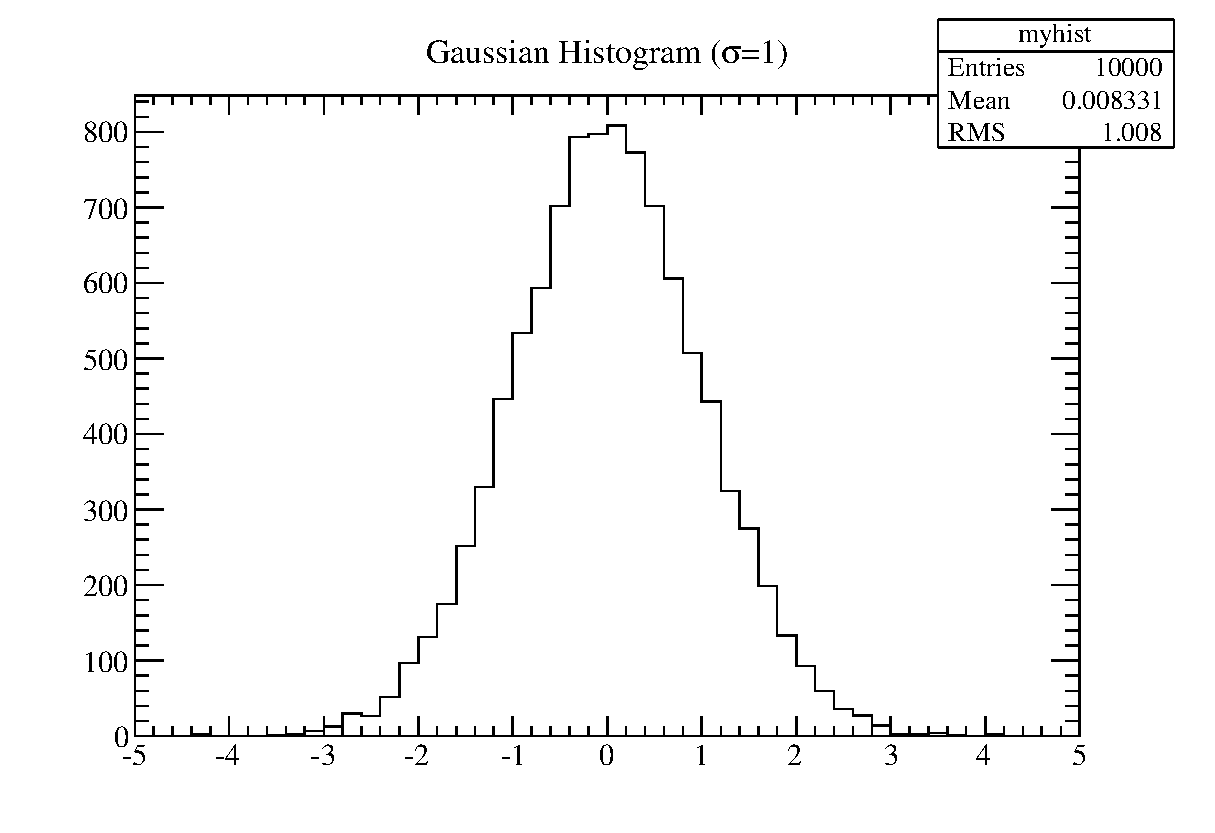
\includegraphics[width=12cm,clip]{fig/first_script_mod.eps}
  \caption{\texttt{\~{}/.rootlogon.C}を使って図\ref{fig_first_script_pdf}の見栄えを変更したもの}
  \label{fig_first_script_mod_eps}
\end{figure}
